\section{Ý tưởng thực hiện}
\subsection{Thuật toán K-Means clustering.}
\subsection{Mục tiêu của K-Means}
K-means clustering là một trong những thuật toán cơ bản nhất trong  học không giám sát (Unsupervised learning). Thuật toán này dùng để phân dữ dữ liệu đầu vào thành các cụm (cluster) khác nhau sao cho dữ liệu trong cùng một cụm có tính chất giống nhau \cite{K-meansClustering}

\subsection{Ý tưởng cơ bản}
Thuật toán gồm 2 bước chính được lặp đi lặp lại cho đến khi đạt được kết quả tối ưu:
\begin{enumerate}
	\item Gán mỗi điểm dữ liệu vào cụm gần nhất với nó.
	\item Tính toán lại tâm của các cụm dựa trên các điểm dữ liệu đã được gán.
	\item Lặp lại bước 1 và 2 cho đến khi không có sự thay đổi nào trong việc gán cụm hoặc đạt đến một số lần lặp tối đa.
\end{enumerate}

\subsection{Mô tả thuật toán}
Ta có thể mô tả thuật toán K-Means clustering qua các bước sau:
\begin{enumerate}
	\item Ta có tập dữ liệu ban đầu như sau:
	      \begin {center}
	      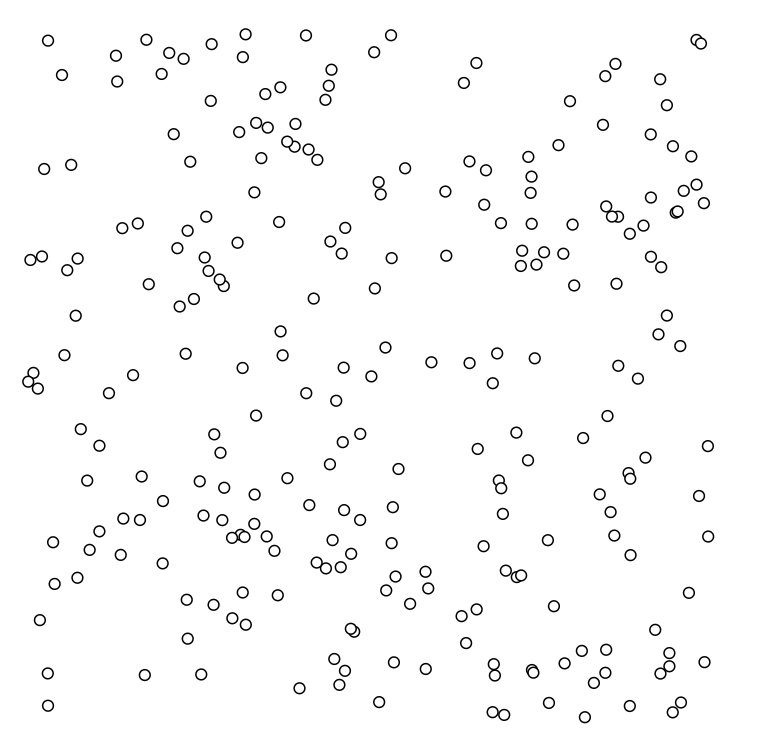
\includegraphics[width=0.5\textwidth]{images/KMeanStep/1.PNG}
	      \end{center}

	\item Chọn ngẫu nhiên $K$ điểm làm tâm của các cụm  phân loại dữ liệu vào từng nhóm. Giả sử ta chọn $K = 3$:
	      \begin{center}
		      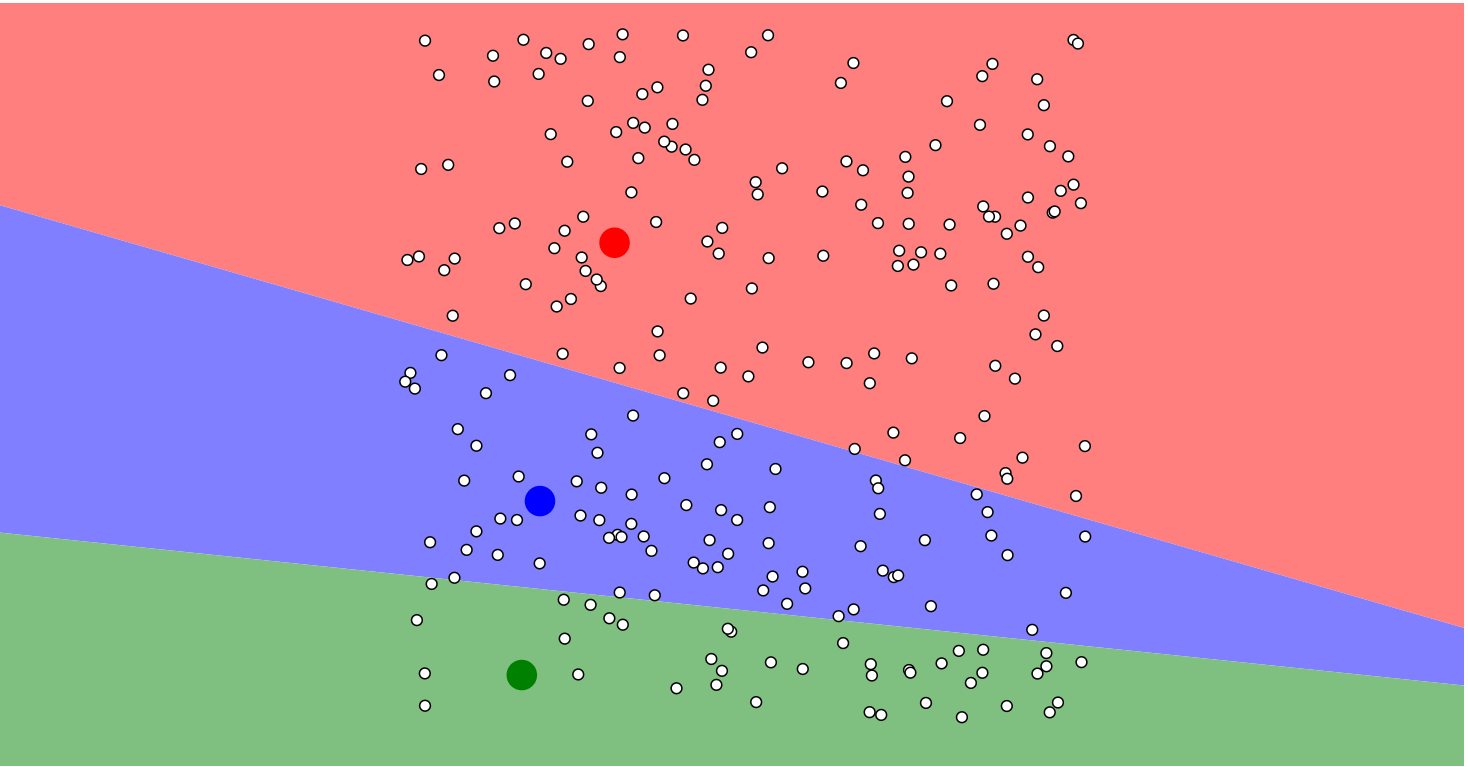
\includegraphics[width=0.8\textwidth]{images/KMeanStep/2.PNG}
	      \end{center}

	\item Gán mỗi điểm dữ liệu vào cụm gần nhất với nó. Khoảng cách giữa các điểm dữ liệu và tâm cụm được tính bằng khoảng cách Euclid:
	      \begin {center}
	      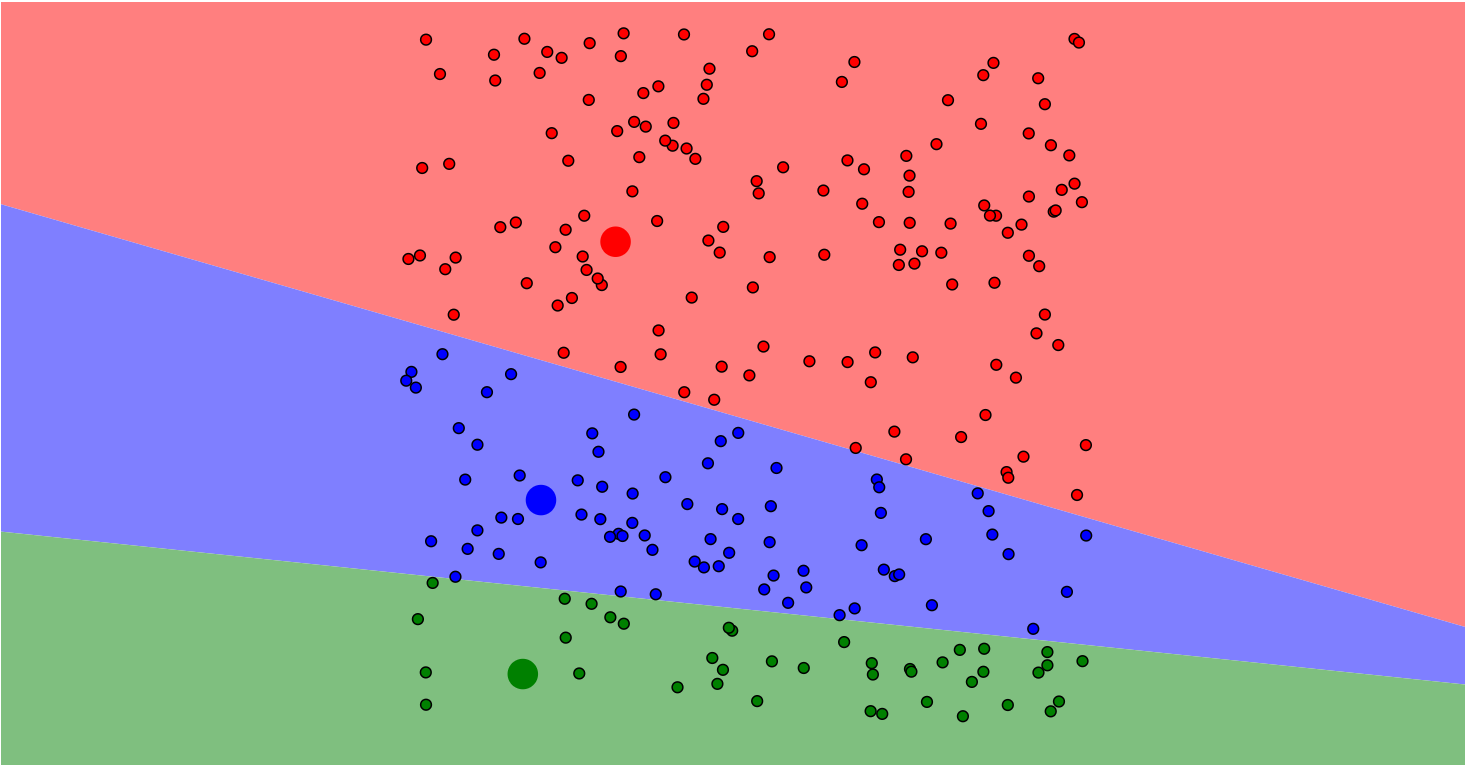
\includegraphics[width=0.8\textwidth]{images/KMeanStep/3.PNG}
	      \end{center}
	\item Tính toán lại tâm của các cụm dựa trên các điểm dữ liệu đã được gán. Tâm cụm mới sẽ là trung bình của tất cả các điểm dữ liệu trong cụm đó:
	      \begin{center}
		      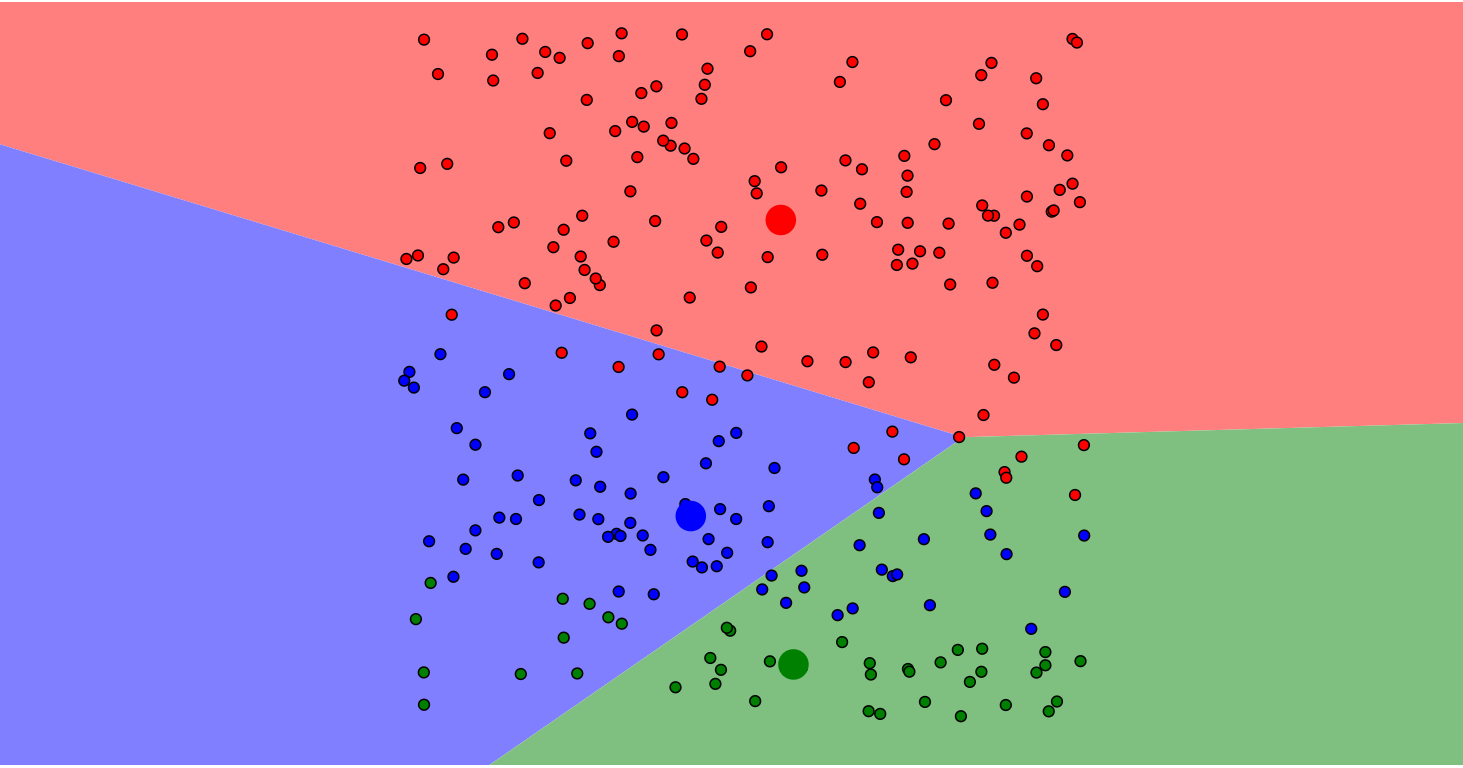
\includegraphics[width=0.8\textwidth]{images/KMeanStep/4.PNG}
	      \end{center}
	\item Lặp lại bước 3 và 4 cho đến khi không có sự thay đổi nào trong việc gán cụm hoặc đạt đến một số lần lặp tối đa. Sau một vài lần lặp, ta có thể thu được kết quả cuối cùng như sau:
	      \begin {center}
	      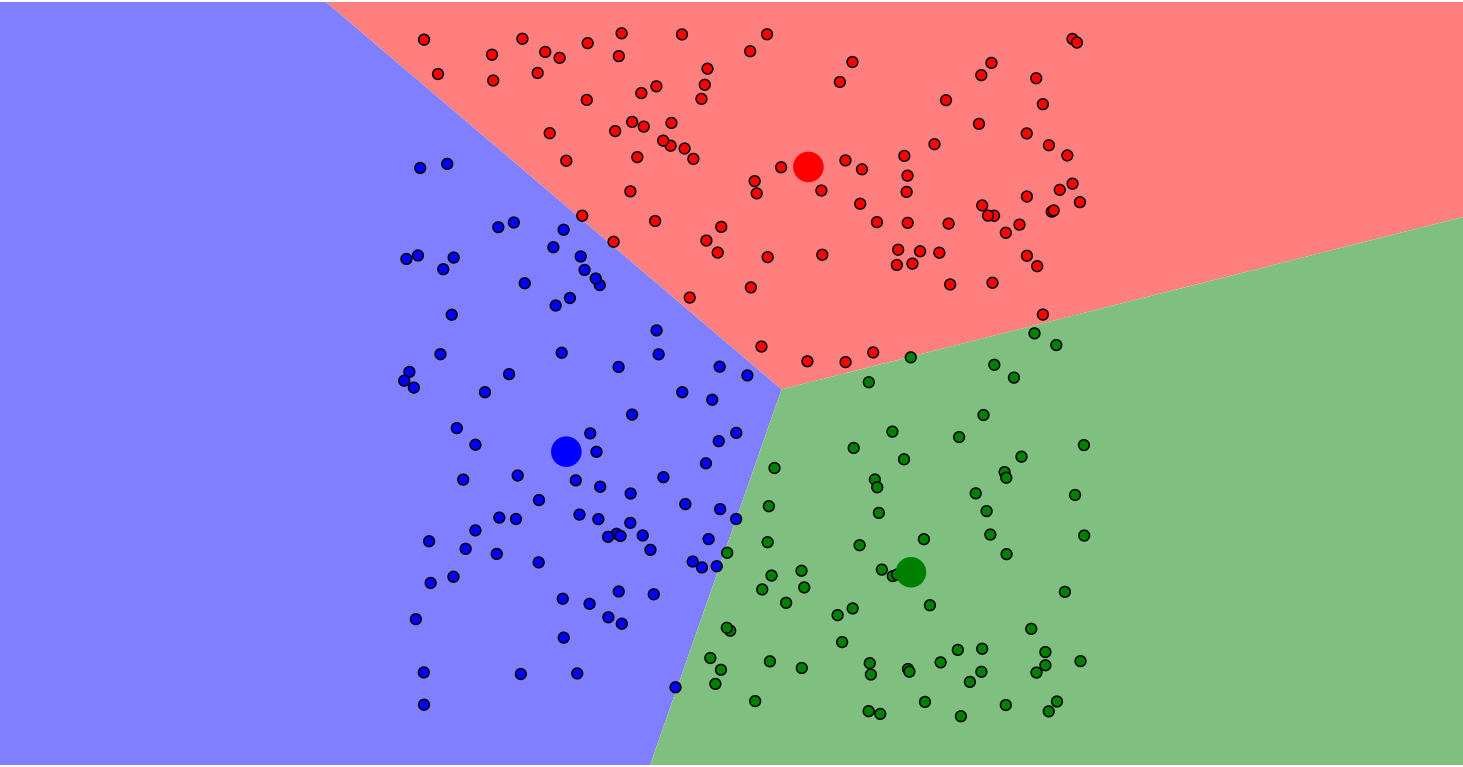
\includegraphics[width=0.8\textwidth]{images/KMeanStep/5.PNG}
	      \end{center}
	\item Kết quả cuối cùng là các cụm dữ liệu được phân loại rõ ràng, với mỗi điểm dữ liệu thuộc về một cụm duy nhất

\end{enumerate}

\subsection{Ứng dụng thuật toán K-Means clustering trong giảm màu ảnh.}

Dựa vào ý tưởng cơ bản của thuật toán K-Means clustering bên trên, ta có thể áp dụng nó để giảm số lượng màu sắc có trong ảnh mà vẫn giữa được các đặc trưng của ảnh ban đầu.

\begin{enumerate}
	\item Đầu tiên, ta sẽ đọc ảnh và chuyển đổi nó từ định dạng 2D (height, width, channels) sang định dạng 1D (height $\times$ width, channels) để dễ dàng xử lý.
	\item Tiếp theo, chọn số lượng màu sắc $K$ mà ta muốn giữ lại trong ảnh.
	\item Tạo ra $K$ điểm centroids từ hình ảnh. Có 2 phương pháp để tạo ra các điểm này:
	      \begin{itemize}
		      \item \texttt{random:} Chọn ngẫu nhiên $K$ điểm centroids trong đoạn từ [0, 255] cho mỗi kênh màu (R, G, B).
		      \item \texttt{in\_pixels:} Chọn ngẫu nhiên $K$ điểm centroids từ các màu sắc có trong ảnh.
	      \end{itemize}
	\item Sử dụng thuật toán K-Means clustering để phân loại các điểm dữ liệu (màu sắc) vào các cụm dựa trên khoảng cách Euclid đến các điểm centroids.
	\item Tính toán lại các điểm centroids dựa trên các điểm dữ liệu đã được phân loại.
	\item Lặp lại bước 4 và 5 cho đến khi không có sự thay đổi nào trong việc gán cụm hoặc đạt đến một số lần lặp tối đa.
	\item Cuối cùng, tạo ra một ảnh mới từ các điểm centroids đã được tính toán. Mỗi điểm dữ liệu trong ảnh ban đầu sẽ được thay thế bằng màu sắc của điểm centroid gần nhất.
\end{enumerate}